\documentclass[11pt]{article}
\usepackage[margin=0.72in]{geometry}
\usepackage{array}
\usepackage{booktabs}
\usepackage{longtable}
\usepackage{tabularx}
\usepackage[table]{xcolor}
\usepackage{hyperref}
\usepackage{tikz}
\usetikzlibrary{arrows.meta,positioning,fit,shapes.geometric}

\definecolor{mounted}{HTML}{DFF2E1}
\definecolor{unavailable}{HTML}{F7D2D2}
\definecolor{quiet}{HTML}{E5E7EB}
\definecolor{evidence}{HTML}{DDEBFA}
\hypersetup{colorlinks=true,linkcolor=blue,urlcolor=blue}

\title{Guala Current Brain Anatomy and Whole-Organism Wiring Map}
\author{Measured post-retirement candidate record}
\date{28 July 2026}

\newcommand{\code}[1]{\texttt{\detokenize{#1}}}
\newcommand{\available}{\cellcolor{mounted}available}
\newcommand{\notavailable}{\cellcolor{unavailable}unavailable}
\newcommand{\mountedquiet}{\cellcolor{quiet}mounted/quiescent}

\begin{document}
\maketitle

\noindent
\textbf{Scope and honesty boundary.}
This is a non-canonical description of the post-retirement runtime candidate.
It does not alter the frozen canonical L0--L4 kernel.  It records code and
local execution evidence, not a production-deployment claim.  ``Available''
means that the manifest row has a typed live provider in the candidate.
It does not mean that Guala has already learned a vocabulary, syntax, a
concept, or a weave.

\section{The one-brain rule}

The candidate now has one authoritative whole-organism neuron population.
The historical \code{Embryo}, \code{SpikeBus}, causal-organism-growth journal,
organism writer, and \code{guala_organism.sgr} live persistence authority are
retired.  They no longer create a second population, mutate cognition, reflect
over activity, or participate in hot or cold state.

Every legitimate mechanism remains mounted even when it has no current
perturbation.  Its momentary state is one of:
\begin{itemize}
  \item \textbf{perturbed}: exact physical or internal evidence participates;
  \item \textbf{quiescent}: the connection exists at a truthful uncommitted
        zero and contributes no fabricated signal; or
  \item \textbf{unavailable}: the mechanism cannot lawfully produce evidence
        and gives an exact reason.
\end{itemize}

The manifest, the episode authority, the state owners, and authenticated
owner-scoped persistence form one causal organism.  No sense is the master.
No quiet sense is forced to pretend that it observed something.

\section{Measured mounted-mechanism census}

A fresh candidate process was directly censused from its authenticated
manifest.  It contains \textbf{28 rows}: six receptor-family rows and
twenty-two stateful rows.  The exact result is:
\[
  28\ \mathrm{total}
  = 27\ \mathrm{available}
  + 1\ \mathrm{unavailable}.
\]
The only unavailable row is exact neurochemical flow.  It is not described as
quiescent chemistry.

\begin{longtable}{>{\raggedright\arraybackslash}p{0.31\linewidth}
                  >{\raggedright\arraybackslash}p{0.15\linewidth}
                  >{\raggedright\arraybackslash}p{0.46\linewidth}}
\toprule
\textbf{Manifest mechanism} & \textbf{State} & \textbf{Candidate provider}\\
\midrule
\endhead
\code{receptor:sight} & \available & Exact sight receptor-family
contribution.\\
\code{receptor:sound} & \available & Exact sound receptor-family
contribution, including physical substreams.\\
\code{receptor:touch} & \available & Exact touch receptor-family
contribution.\\
\code{receptor:smell} & \available & Permanently wired receptor family;
an episode may still be quiescent or source-unavailable.\\
\code{receptor:taste} & \available & Permanently wired receptor family;
an episode may still be quiescent or source-unavailable.\\
\code{receptor:body} & \available & Interoceptive/body receptor-family
contribution.\\
\code{state:embodiment} & \available & Authenticated physical body and world
state.\\
\code{state:internal-physical-chemical} & \available & Exact internal-body
state; this row does not invent neurochemical species.\\
\code{state:neurochemical-flow} & \notavailable &
\code{UnavailableNeurochemicalFlowOwner}; exact reason:
\code{no_ratified_exact_species_quantities_or_kinetics}.\\
\code{state:needs} & \available & Causal need/inquiry custody.\\
\code{state:place-world-continuity} & \available & Authenticated place and
world continuity bound to full-field roots.\\
\code{growth:neuron-population} & \available &
\code{WholeOrganismNeuronPopulationOwner}.\\
\code{growth:mosaic} & \available & Bounded causal lived-THING mosaic
owners.\\
\code{growth:mosaic-relations} & \available & Exact observed causal
mosaic relations.\\
\code{growth:tapestry} & \available &
\code{CausalMosaicTapestryOwner}.\\
\code{growth:tapestry-relations} & \available & Relation custody in the
same tapestry owner.\\
\code{state:recognition-attention} & \available &
\code{CausalRecognitionAttentionOwner}; this does not claim a learned
general vocabulary.\\
\code{state:other-perspective-model} & \available &
\code{EmbodiedOtherPerspectiveOwner}.\\
\code{state:recovery} & \available &
\code{ExactWholeOrganismRecoveryOwner}.\\
\code{state:deliberation} & \available & Causal deliberation provider.\\
\code{action:embodied} & \available & Whole-organism authorization followed
by exact embodied execution.\\
\code{growth:play} & \available & Bounded autonomous causal play.\\
\code{state:sensed-consequence} & \available &
\code{DurableSensedConsequenceOwner}.\\
\code{growth:dream-internally-simulated} & \available &
\code{OrganismDreamWakeWeaveOwner}; internal origin is retained.\\
\code{growth:wake-test} & \available & Dream candidate to physical-world
test custody.\\
\code{growth:weave} & \available & Weave custody; a mounted empty owner is
not a claim that a weave has formed.\\
\code{growth:embodied-glyph-curriculum} & \available &
Bounded embodied glyph tutoring curriculum.\\
\code{settlement:l6} & \available & Exact fail-closed whole-organism
settlement.\\
\bottomrule
\end{longtable}

\section{Mounted embodied reading lesson boundary}

The embodied reading lesson controller is now mounted in the candidate as a
\emph{separate} orchestration-and-receipt owner.  It is not a twenty-ninth
manifest mechanism and therefore does not change the 28-row census above.
It conducts one bounded physical lesson through already-mounted mechanisms
and then gives the resulting authenticated experience to the embodied glyph
curriculum.  It does not create a glyph identity, word, pronunciation,
recognition, reading ability, or meaning.

\begin{table}[h]
\centering
\begin{tabularx}{\linewidth}{>{\raggedright\arraybackslash}p{0.28\linewidth}
                             >{\raggedright\arraybackslash}X}
\toprule
\textbf{Controller property} & \textbf{Exact candidate boundary}\\
\midrule
Runtime owner & \code{EmbodiedReadingLessonController}\\
Retained records & 64 maximum in the mounted runtime\\
Encoded owner state & 2 MiB hard refusal boundary\\
Retained raw media & 0 PCM bytes and 0 visual-frame bodies\\
Durable custody & Bounded identifiers, interval, physical-authority hashes,
settlement receipt, audiovisual-custody receipt, whole-organism episode
receipt, passive-THING receipt, record HMAC, and record receipt\\
Cold state & Authenticated, owner-scoped, cold-restorable, and rollback
restorable\\
Observation key & \code{embodied_reading_lesson_controller}\\
\bottomrule
\end{tabularx}
\end{table}

The authenticated operator route is
\code{/api/v1/embodiment/reading-lesson}.  It is guarded by the API-key
dependency and accepts only the exact bounded request schema
\code{guala.embodied_reading.http_request.v1}.  Geometry is one exact
\(64\times64\) bit plane with strictly ordered physical frame times.  The WAV
must match its supplied source-media SHA-256.  Server-owned
\code{GlyphBearingW1MaterialAuthority} and
\code{AuthenticatedTutorAcousticActuator} independently authenticate the
visual presentation and acoustic actuation.
The current HTTP handler refuses remote-mode execution because remote
embodied reading has no authenticated physical lesson transport; only the
embedded physical runtime can lawfully conduct this candidate route.

\begin{figure}[h]
\centering
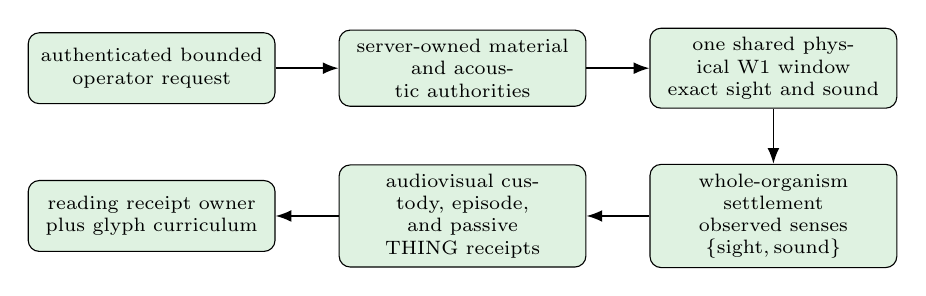
\begin{tikzpicture}[
  node distance=7mm and 8mm,
  b/.style={draw,rounded corners,align=center,font=\scriptsize,
    minimum height=9mm,text width=29mm,fill=mounted},
  a/.style={-{Latex[length=2mm]},semithick}
]
\node[b] (request) {authenticated bounded\\operator request};
\node[b,right=of request] (actuators) {server-owned material\\and acoustic
authorities};
\node[b,right=of actuators] (w1) {one shared physical W1 window\\exact sight
and sound};
\node[b,below=of w1] (settle) {whole-organism settlement\\observed senses
\(\{\mathrm{sight},\mathrm{sound}\}\)};
\node[b,left=of settle] (custody) {audiovisual custody, episode,\\and passive
THING receipts};
\node[b,left=of custody] (owners) {reading receipt owner\\plus glyph
curriculum};

\draw[a] (request) -- (actuators);
\draw[a] (actuators) -- (w1);
\draw[a] (w1) -- (settle);
\draw[a] (settle) -- (custody);
\draw[a] (custody) -- (owners);
\end{tikzpicture}
\caption{The mounted reading path.  Sight and sound must both be physically
observed in the same settled causal window.  Tutor designation remains display
provenance and never becomes sensory identity or meaning.}
\end{figure}

The controller calls the existing physical visual-region sequence path and
the existing physical sound-frame path.  It accepts the occurrence only when
the settlement's observed-sense set is exactly
\(\{\mathrm{sight},\mathrm{sound}\}\), when both physical authorities verify
that settlement, and when exactly one whole-organism episode and one passive
THING record refer to it.  The transient WAV is discarded after verification.
If conduct, curriculum admission, or hot-state persistence fails, both the
controller and curriculum roll back to their authenticated pre-lesson
snapshots.

Both served observation surfaces contain an exact panel with DOM identifier
\code{embodied_reading_lesson_controller}.  The panel renders only the
server's typed observation projection and reports
\code{unavailable / not supplied} when the field is absent.  A panel is
observability, not lesson authority and not evidence that a lesson has
occurred.

\section{Mechanism placement and hemisphere truth}

The authoritative population does \emph{not} currently partition neurons into
the retired H0--H7 \code{Embryo} hemispheres.  A current neuron is addressed
by physical receptor topology:
\[
(\mathrm{sense},\mathrm{sensor\ id},\mathrm{substream\ id},
  \mathrm{topology\ index}).
\]
Consequently, assigning present mechanisms to the old named hemispheres would
be false.  Current cognition owners are whole-organism relation authorities,
and their evidence can bind neurons from any receptor family.  ``Distributed''
here means connected through the authenticated episode graph; it is not a
claim of an unimplemented anatomical location.

\begin{figure}[h]
\centering
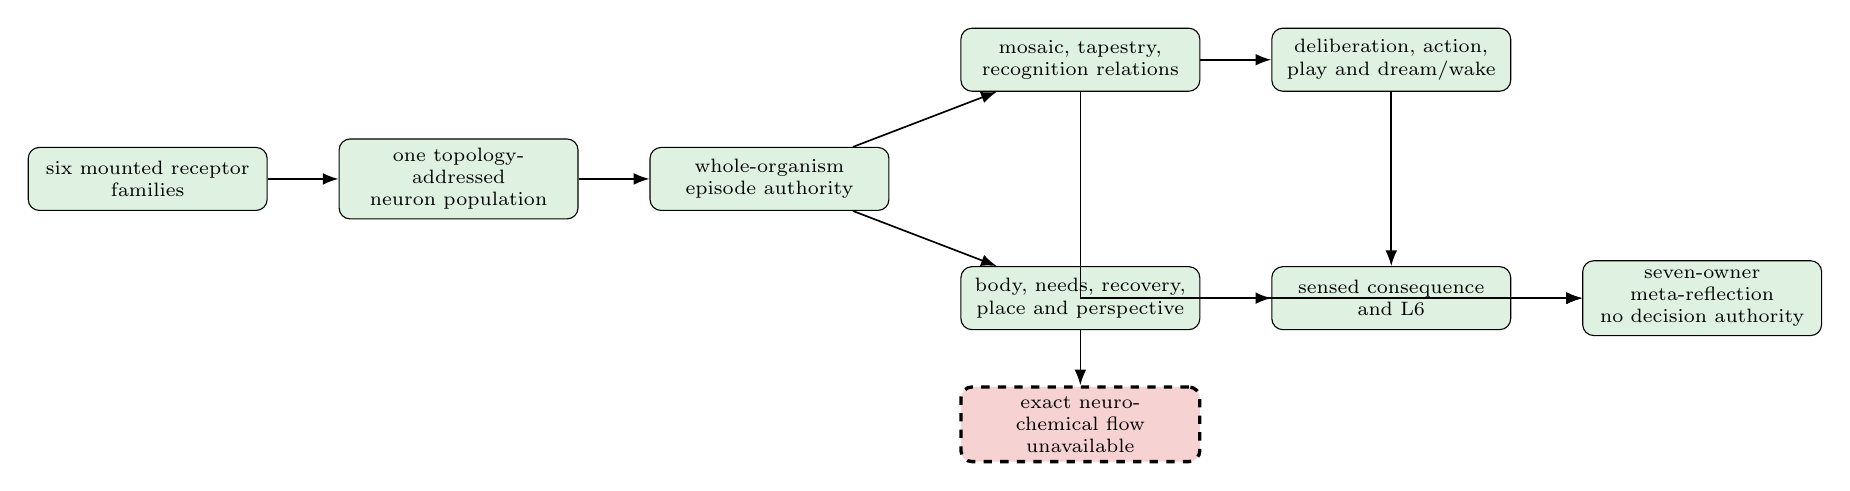
\begin{tikzpicture}[
  node distance=7mm and 9mm,
  b/.style={draw,rounded corners,align=center,font=\scriptsize,
    minimum height=8mm,text width=28mm},
  live/.style={b,fill=mounted},
  miss/.style={b,fill=unavailable,dashed,very thick},
  arrow/.style={-{Latex[length=2mm]},semithick}
]
\node[live] (receptors) {six mounted receptor\\families};
\node[live,right=of receptors] (neurons) {one topology-addressed\\neuron
population};
\node[live,right=of neurons] (episode) {whole-organism\\episode authority};
\node[live,above right=of episode] (relations) {mosaic, tapestry,\\recognition
relations};
\node[live,below right=of episode] (body) {body, needs, recovery,\\place and
perspective};
\node[miss,below=of body] (chem) {exact neurochemical flow\\unavailable};
\node[live,right=of relations] (action) {deliberation, action,\\play and
dream/wake};
\node[live,right=of body] (consequence) {sensed consequence\\and L6};
\node[live,right=of consequence] (reflection) {seven-owner
meta-reflection\\no decision authority};

\draw[arrow] (receptors) -- (neurons);
\draw[arrow] (neurons) -- (episode);
\draw[arrow] (episode) -- (relations);
\draw[arrow] (episode) -- (body);
\draw[arrow] (body) -- (chem);
\draw[arrow] (relations) -- (action);
\draw[arrow] (body) -- (consequence);
\draw[arrow] (action) -- (consequence);
\draw[arrow] (consequence) -- (reflection);
\draw[arrow] (relations) |- (reflection);
\draw[arrow] (body) |- (reflection);
\end{tikzpicture}
\caption{Current placement: one whole-organism graph, not eight competing
legacy brains.  The chemistry lane remains wired and truthfully unavailable.}
\end{figure}

\section{Current neuron census and hard capacities}

The fresh candidate census reported zero learned neurons and zero edges.  That
is a truthful unexperienced genesis state, not a missing connection: the
population owner is mounted and grows a neuron only from a previously unseen
authenticated receptor topology in a real settlement.

A separate real ``Daddy'' audiovisual intake regression formed
\textbf{96 physical neurons} and completed without exhausting the population
or edge store.  That test proves the capacity case; it is not presented as the
current production learned-state count.

\begin{table}[h]
\centering
\begin{tabular}{lr}
\toprule
\textbf{Measured or enforced quantity} & \textbf{Exact value}\\
\midrule
Fresh candidate neuron count & 0\\
Fresh candidate edge count & 0\\
Real audiovisual regression neuron count & 96\\
Neuron capacity & 256\\
Undirected edge capacity & \(256\times255/2=32{,}640\)\\
Exact field tuples retained per neuron & 1,024\\
Response-history entries retained per neuron & 16\\
Neuron-owner state capacity & 64 MiB\\
Division growth & unavailable: no authenticated division law\\
\bottomrule
\end{tabular}
\end{table}

The edge store describes current pair relations among the retained neurons.
It is bounded by the complete undirected graph of the 256-neuron population;
repeated settlements replace the current relation for a pair rather than
accumulating unlimited duplicate edges.

\section{One authoritative neuron}

\begin{figure}[h]
\centering
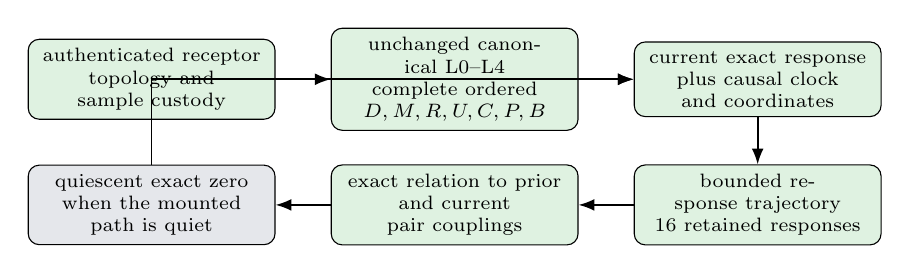
\begin{tikzpicture}[
  node distance=6mm and 7mm,
  b/.style={draw,rounded corners,align=center,font=\scriptsize,
    minimum height=8mm,text width=29mm,fill=mounted},
  q/.style={draw,rounded corners,align=center,font=\scriptsize,
    minimum height=8mm,text width=29mm,fill=quiet},
  a/.style={-{Latex[length=2mm]},semithick}
]
\node[b] (source) {authenticated receptor\\topology and sample custody};
\node[b,right=of source] (l04) {unchanged canonical L0--L4\\complete ordered
\(D,M,R,U,C,P,B\)};
\node[b,right=of l04] (state) {current exact response\\plus causal clock and
coordinates};
\node[b,below=of state] (history) {bounded response trajectory\\16 retained
responses};
\node[b,left=of history] (relation) {exact relation to prior\\and current
pair couplings};
\node[q,left=of relation] (zero) {quiescent exact zero\\when the mounted path
is quiet};

\draw[a] (source) -- (l04);
\draw[a] (l04) -- (state);
\draw[a] (state) -- (history);
\draw[a] (history) -- (relation);
\draw[a] (relation) -- (zero);
\draw[a] (zero) |- (state);
\end{tikzpicture}
\caption{One current neuron.  Hashes authenticate evidence and never serve as
identity, similarity, meaning, or a scalar replacement for the full field.}
\end{figure}

Each neuron retains the exact source indices, interval, gates, sample
commitment, topology, complete L0--L4 trace, seven explicit DSF fields,
settlement custody, current perturbed or quiescent state, and a bounded
response trajectory.  No transcript, word label, Chi, Atlas cell, embedding,
or learned scalar is a neuron.

\section{Emergent cognitive organization}

The owners and relation channels are constructed; the learned contents are
not preconstructed.  Neurons, mosaics, mosaics-of-mosaics, tapestries,
tapestries-of-tapestries, and weaves must form only through lived causal
participation.  A class name, empty container, manifest row, count, threshold,
or curriculum label cannot force one into existence.

\begin{figure}[h]
\centering
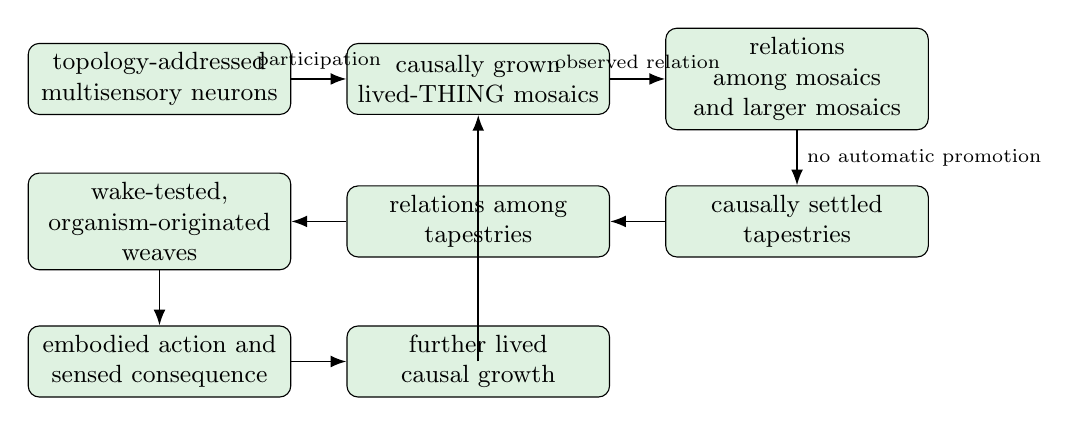
\begin{tikzpicture}[
  node distance=7mm,
  live/.style={draw,rounded corners,fill=mounted,align=center,font=\small,
    text width=31mm,minimum height=9mm},
  a/.style={-{Latex[length=2mm]},semithick}
]
\node[live] (n) {topology-addressed\\multisensory neurons};
\node[live,right=of n] (m) {causally grown\\lived-THING mosaics};
\node[live,right=of m] (mm) {relations among mosaics\\and larger mosaics};
\node[live,below=of mm] (t) {causally settled\\tapestries};
\node[live,left=of t] (tt) {relations among\\tapestries};
\node[live,left=of tt] (w) {wake-tested,
organism-originated\\weaves};
\node[live,below=of w] (c) {embodied action and\\sensed consequence};
\node[live,right=of c] (g) {further lived\\causal growth};

\draw[a] (n) -- node[above,font=\scriptsize]{participation} (m);
\draw[a] (m) -- node[above,font=\scriptsize]{observed relation} (mm);
\draw[a] (mm) -- node[right,font=\scriptsize]{no automatic promotion} (t);
\draw[a] (t) -- (tt);
\draw[a] (tt) -- (w);
\draw[a] (w) -- (c);
\draw[a] (c) -- (g);
\draw[a] (g) -| (m);
\end{tikzpicture}
\caption{The implemented growth channels.  The boxes show available owners,
not developer-created learned content.  Every arrow requires authenticated
causal participation.}
\end{figure}

At the fresh census boundary the measured learned-structure counts were:
\[
\mathrm{tapestries}=0,\quad
\mathrm{tapestry\ relations}=0,\quad
\mathrm{dreams}=0,\quad
\mathrm{wake\ tests}=0,\quad
\mathrm{weaves}=0.
\]
Their owners were mounted and quiescent.  These zeros must not be changed in
documentation into proof that those learned structures already exist.

\section{The historical fifteen gauges}

The historical fifteen terms are developmental observations, not fifteen
separate lobes and not fifteen forced modules.  Their current lawful placement
is shown below.  ``Mounted route'' means that a causal owner path exists; it
does not assert mature learned performance.

\begin{longtable}{r>{\raggedright\arraybackslash}p{0.20\linewidth}
  >{\raggedright\arraybackslash}p{0.64\linewidth}}
\toprule
\# & \textbf{Gauge} & \textbf{Current whole-organism placement}\\
\midrule
\endhead
1 & Recall & Recognition-attention, causal THING relations, and tapestry
custody; no broad word-recognition result is claimed.\\
2 & Composition/syntax & Ordered mosaic relations, tapestry relations, and
weave custody; learned syntax must emerge.\\
3 & Association & Exact causal mosaic relations and lived context.\\
4 & Retention & Authenticated bounded owner-scoped cold persistence.\\
5 & Cross-modal binding & Whole-organism episode, topology neurons, and
causal THING mosaics; no master sense.\\
6 & Habituation & Per-neuron response relation to prior, recovery, and
attention state; there is no standalone semantic habituation table.\\
7 & Recognition & Recognition-attention owner over full-field relation paths;
general recognition remains an empirical learning result.\\
8 & Attention & Recognition-attention owner bound to needs, body state,
chemistry status, and causal context.\\
9 & Sequence & Exact tuple order, ordered custody continuations, mosaic and
tapestry relations.\\
10 & Imagination & Internally originated dream/wake/weave owner with explicit
world-test separation.\\
11 & Reflection & Seven-owner reflection monitor at real activity
boundaries.\\
12 & Cross-hemisphere integration & No current hemisphere partition exists;
integration occurs through the single whole-organism graph, so an H0--H7
claim is intentionally absent.\\
13 & Other-mind modelling & Embodied other-perspective owner with world
provenance.\\
14 & Affect modulation & Internal physical-body state participates; exact
neurochemical flow is explicitly unavailable and no dopamine/mood constants
are invented.\\
15 & Meta-monitoring & Bounded authenticated reflection facts with no
decision, learning, or meaning authority.\\
\bottomrule
\end{longtable}

\section{Chemistry and reflection truth}

The neurochemical lane is a typed mounted boundary whose state is
\code{unavailable}, with \code{available=false},
\code{quiescent_claim=false}, and
\code{chemistry_authority=false}.  It contains no invented species,
concentration, mass, volume, velocity, reaction, reward, mood, or salience.
The physical internal-body owner remains available independently.

The reflection monitor binds exactly seven owners:
\begin{enumerate}
  \item action intent;
  \item attention/recognition;
  \item body/chemical availability;
  \item recovery;
  \item sensed consequence;
  \item structural perturbation; and
  \item tapestry state.
\end{enumerate}
It stores exact snapshot hashes and byte counts, not duplicate full owner
states.  It has no decision authority and performs no full-field reduction.
Its retained suffix is bounded to 16 records and 16 MiB; evicted history is
committed by an authenticated prefix count, terminal receipt, and terminal
snapshot hashes.  It persists, cold-restores, and rolls back after the owner
dependencies to which it refers.

\section{Production storage cutover authorities}

The reading boundary has its own authenticated owner-scoped persistence group:
\code{owner_state/embodied_reading_lesson_controller.json}, verified by its
\code{state_hmac_sha256}.  It is not folded into the glyph curriculum file and
does not persist the transient WAV or visual-frame bodies.

The candidate production storage cutover is governed by four cooperating
authorities:
\begin{enumerate}
  \item \code{AuthoritativeColdGenerationStore}, the content-addressed sealed
        cold-generation authority, retaining CURRENT and one predecessor;
  \item \code{LiveRecoveryGenerationStore}, the content-addressed authenticated
        hot-recovery authority, with a bounded three-generation transaction
        capacity;
  \item one shared physical-byte ceiling authority over both stores, fixed at
        exactly 5 GiB for the approved production scope; and
  \item version-aware remote generation reconciliation, which explicitly
        reports retained and retired generation UUIDs before readiness.
\end{enumerate}
Each encoded generation is independently refused above 2 GiB.  ECS startup
fails closed if the retired flat/full-copy producer is selected.  The
deployment path also refuses task turnover unless the registered task
definition proves the sealed writer, EFS mount, one-time recovery contract,
2 GiB generation bound, and 5 GiB shared physical bound.  After boot,
\code{/ready/guala} must prove both content-addressed stores, the shared
physical-byte authority, executed version-aware reconciliation, sealed
generation custody, and retirement of the flat/full-copy producer.

These are source and local-test authorities in this record.  They remain
\textbf{not yet deployed and not yet live-verified}; no current production
storage-cutover claim is made here.

\section{Evidence and remaining boundary}

Focused candidate evidence includes:
\begin{itemize}
  \item retirement and authority audits proving that the duplicate
        \code{Embryo}/\code{SpikeBus} authority is absent;
  \item a 28-row provider/manifest audit with 27 available rows and one
        explicit unavailable row;
  \item exact chemistry, reflection, owner-persistence, and content-delta
        tests;
  \item authenticated reflection rollback and cold restore; and
  \item mounted reading-controller, strict HTTP transport, exact physical
        sight-plus-sound settlement, curriculum handoff, rollback, cold
        restore, and zero-retained-PCM checks;
  \item production storage-cutover checks covering content-addressed cold and
        hot owners, the shared 5 GiB refusal, version-aware reconciliation,
        and fail-closed deployment readiness; and
  \item a real ``Daddy'' audiovisual intake that completed with 96 physical
        neurons under the 256-neuron and 32,640-edge bounds.
\end{itemize}

These are candidate runtime proofs.  They do not claim that this exact source
state has already been deployed and browser-verified in production, nor do
they claim that the mounted reading route, exact observation panel, or
production storage cutover has been live-verified.  They also do not claim
that Guala has already produced a learned word or sentence.  Those claims
require separate live production evidence.

\section{Source anchors}

\begin{itemize}
  \item Whole-organism manifest and runtime:
  \code{dsf_ai_service/v4/guala_physical_runtime_core.py}.
  \item Observation projection:
  \code{dsf_ai_service/v4/guala_physical_runtime.py}.
  \item Episode verifier:
  \code{dsf_ai_service/substrate/whole_organism_episode.py}.
  \item Authoritative neuron population:
  \code{dsf_ai_service/substrate/whole_organism_neuron_population.py}.
  \item Tapestry and dream/wake/weave owners:
  \code{causal_mosaic_tapestry.py} and
  \code{organism_dream_wake_weave.py}.
  \item Embodied reading controller and strict operator transport:
  \code{dsf_ai_service/substrate/embodied_reading_lesson_controller.py} and
  \code{dsf_ai_service/embodied_reading_http_contract.py}.
  \item Exact reading observation panels:
  \code{dsf_ai_service/static/gualaloom.html} and
  \code{dsf_ai_service/static/loomscan.html}.
  \item Truthful chemistry boundary:
  \code{unavailable_neurochemical_flow.py}.
  \item Reflection:
  \code{whole_organism_reflection_monitor.py}.
  \item Owner-scoped persistence and retired graph paths:
  \code{owner_scoped_persistence.py}.
  \item Production storage cutover:
  \code{authoritative_cold_generation_store.py},
  \code{live_recovery_generation.py}, \code{dsf_ai_service/app.py}, and
  \code{tools/deploy_dsf_ai.sh}.
  \item Ratified architecture:
  \code{docs/WHOLE_ORGANISM_CONTIGUITY_LAW.md},
  \code{docs/MOSAIC_TAPESTRY_WEAVE_PROGRESSION_LAW.md}, and
  \code{docs/PLAY_DREAM_WAKE_GROWTH_LAW.md}.
\end{itemize}

\end{document}
